\RequirePackage{lineno}
\documentclass[a4paper]{jpconf}
\usepackage{graphicx}
\begin{document}

\linenumbers

\title{Glint: VM image distribution in an OpenStack multi-cloud environment}

\author{A.~Charbonneau, M.~Conklin, R.~Demarais, C.~Driemel, I.~Gable, C.~Leavett-Brown, 
M.~Paterson, R.J~Sobie, R.~Taylor}

\address{University of Victoria, Victoria, Canada}

\ead{rsobie@uvic.ca}

\begin{abstract}
The use of cloud computing is becoming widespread in the HEP community.  
In many instances, individual clouds are being federated to appear as a single
infrastructure that can be connected, for example, to the WLCG.
For a small number of clouds, it is relatively easy to manage the virtual
machine images on all the sites.  
However, as the number of clouds increases, then keeping track of the images
requires a more robust management system.
Glint is designed to manage virtual machine images on OpenStack clouds.
Glint makes it easy to distribute images on multiple clouds in a reliable and
error free manner. 
\end{abstract}

\section{Introduction}

The use of clouds in HEP is becoming a significant source of computing resources 
for MC production and data analysis.
There are a number of compelling reasons for the migration to clouds:
clouds give researchers quick and dynamic access to unused or opportunistic
resources;  sites find it easier to manage multiple project that have their
own specific software requirements; and cloud technology is support by a
large international community of developers.

If a cloud site is colocated with other traditional HEP computing resources or
the resource has been transformed to a cloud, then it can be viewed as another
grid site on the WLCG.
Utilizing opportunistic resources (private non-HEP or commercial) can be done
by directly linking the cloud to the project workload management system (for example,
VMDIRAC \cite{vmdirac}).
Alternatively, one can unify the clouds into a single infrastructure (``grid of clouds'').
The HTCondor/CloudScheduler \cite{chep:gable-talk} or VAC/VCycle \cite{chep:vac-vcycle}
were presented at this conference and are two methods for unifying clouds.
 
We have established a distributed cloud system using HTCondor/CloudScheduler for
particle physics and astronomy applications \cite{hpcs:cloudpaper, sobie-nyc-cloud}.
The distributed cloud is currently used by the ATLAS \cite{ryan-chep} 
and Belle-II \cite{sobie-chep} experiments.
The system is designed to boot user or project-specific virtual machines (VM's),
making it easy to run HTC batch workloads from multiple projects.

The majority of the clouds today are using OpenStack software.
OpenStack clouds require that a user boot an image from the local Glance repository.
If a user wants to use multiple clouds, either manually or with our 
HTCondor/CloudScheduler system, then the image must be manually uploaded 
to the Glance repository of each cloud.
Transfering VM images manually becomes tedious and error prone as one gets access
to more IaaS clouds.
We realized that we required a better way of managing the VM images and we 
developed Glint help us manage VM images over multiple OpenStack clouds.

The Glint service is designed for OpenStack clouds and the Glance repository
with a pluggable architecture to allow support for different cloud types.
Through a web browser or command-line interface, the user can identify clouds 
and control the distribution of images.
Glint is currently used with the distributed cloud systems for ATLAS and Belle-II.
In this paper, we describe the design and implementation of Glint.
The source code is available from the Git repository \cite{glint}.



\section{Design}
Glint is designed to operate as an OpenStack service. The glint service is comprised of 4 components. The service component, which actually pushes and pulls data from different Glance repositories; The GUI component, which provides a user friendly interface integrated with the OpenStack's Horizon dashboard; The Command Line Interface component, which allows users to try out glint without having to change or add another dashboard; And the Application Programming Interface, which allow developers to create their own tools. Figure ~\ref{fig:glintdesign.pdf} depicts a software component model of glint and it's integration with OpenStack. 

\begin{figure}[ht]
\begin{center}
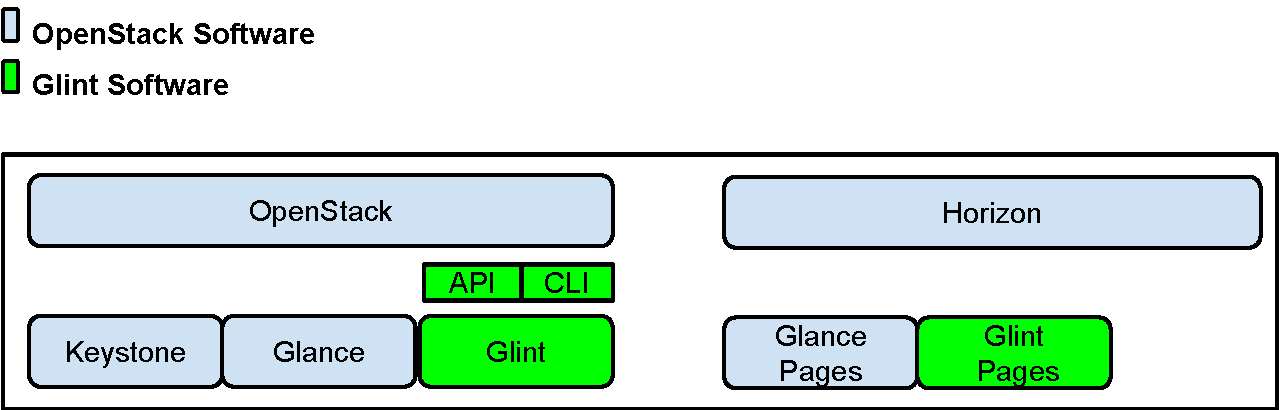
\includegraphics[width=36pc]{images/glintdesign.pdf}
\caption{\label{fig:glintfigure}Glint Software Components}
\end{center}
\end{figure}

There are 3 main services Glint provides; Glint allows users to create remote sites representing a remote glance repository; Glint users can add their remote repository credentials for Glint management; Finally, Glint uses a multithreaded manager to manage image distribution. Image management is the most complicated operation provided by Glint. Figure~\ref{fig:glintseqdiag} depicts the process of moving an image between two sites. 

\begin{figure}[h]
\begin{center}
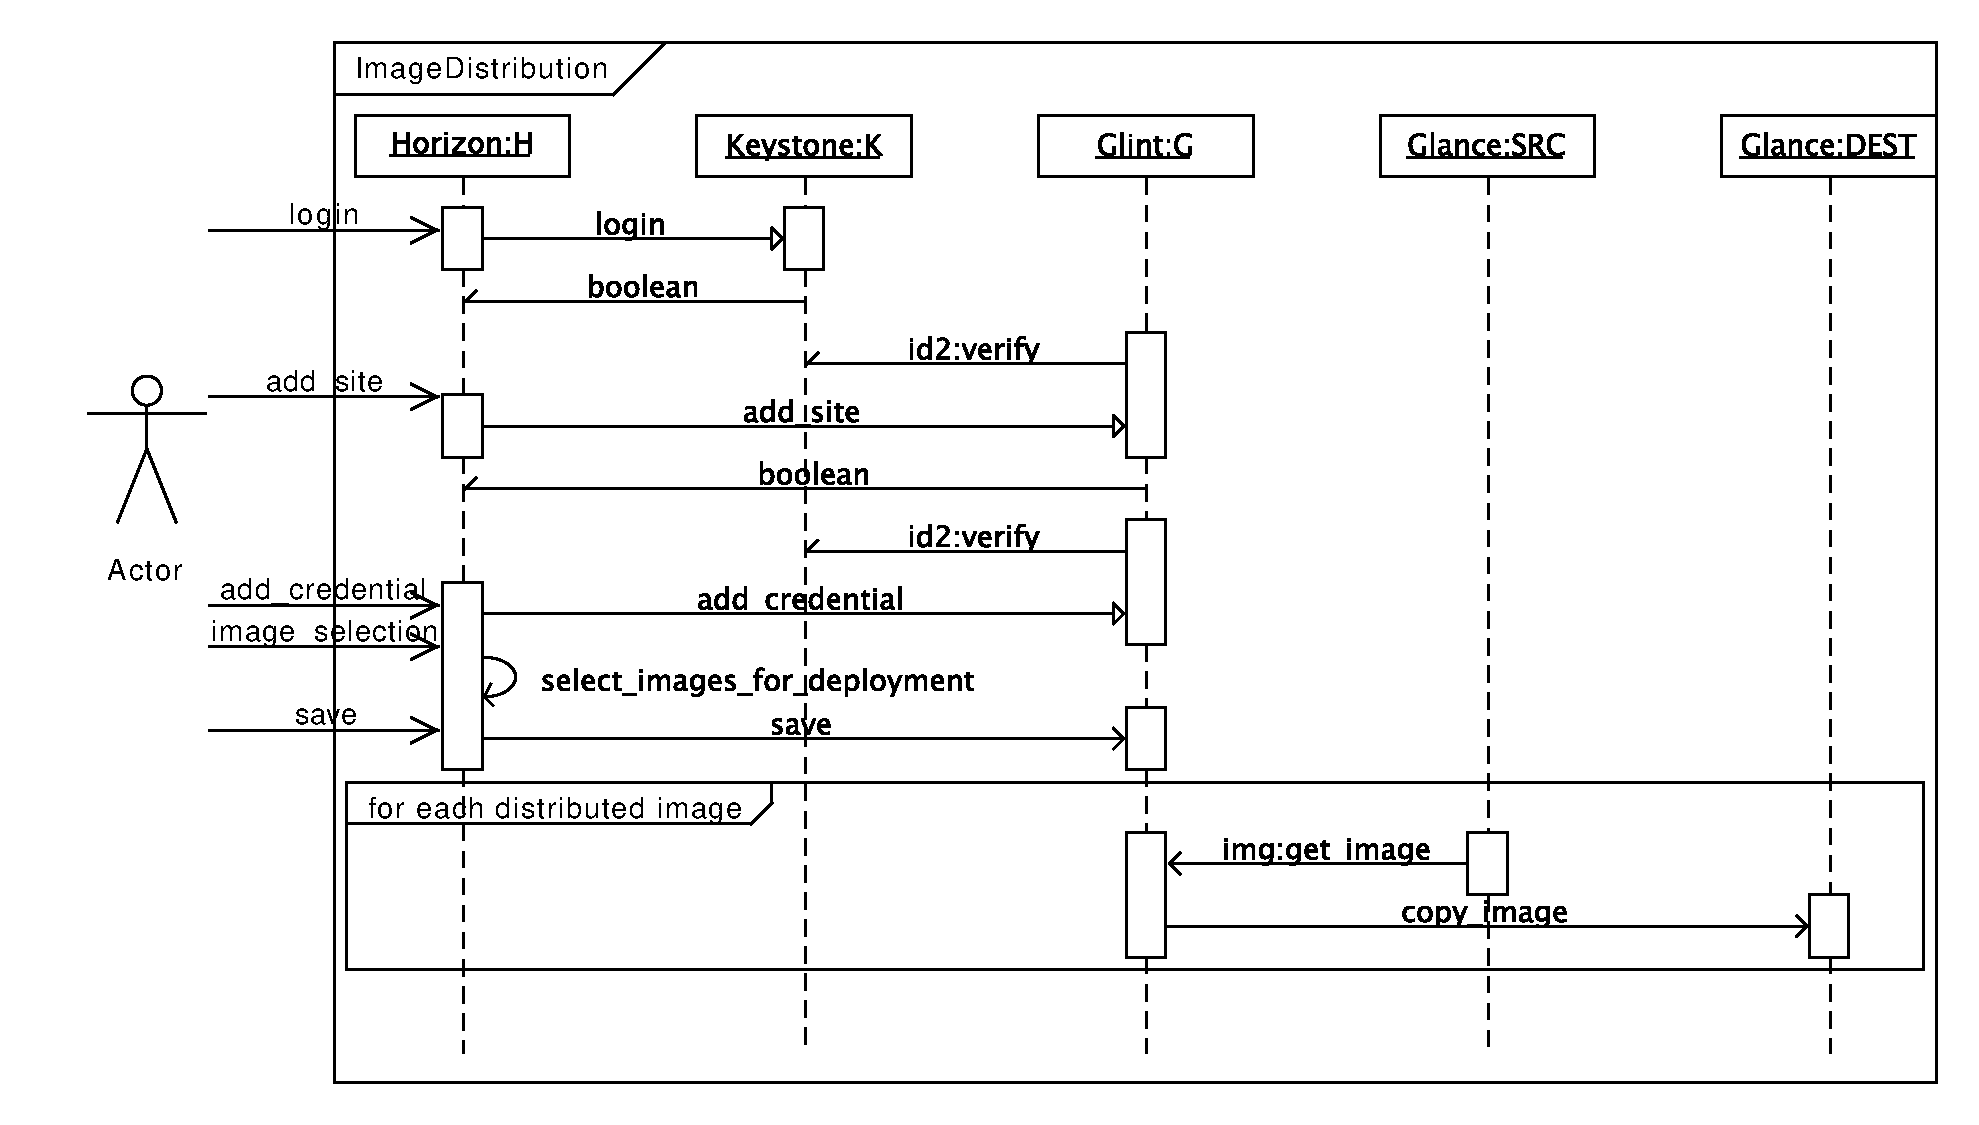
\includegraphics[width=36pc]{images/glintseqdiag.pdf}
\caption{\label{fig:glintseqdiag}Image Distribution Design}
\end{center}
\end{figure}

Glint is designed around OpenStack's Keystone for user authenication. This design requires a user to have an openstack account on the site that Glint is using as its primary host. Therefore the user must login and register with Glint which will then use Keystone to check if the user is valid (c.f., Figure~\ref{fig:glintlogin}). If the user is valid, Keystone will generate an authenication token that the glint service maintains. User requests are then performed on behalf of glint using the token for authentication.

The concepts of remote OpenStack sites and remote site credentials is essential in the design of glint. Users can add remote sites as a source and destination of images. Site credentials can then be added so Glint can use the site without having to request input from the user everytime the site is accessed. Figure~\ref{fig:glintsitecred} depicts the user added a remote site to the glint service.

OpenStack's Glance service provides the image copying and deleting functionality. Glint relies on this service to move images around remote sites. Figure~\ref{fig:glintdist} depicts the image distrubtion process. It requires the user to select which images they want on each site, once the user is happy they can save the new configuration. Glint proceeds to create a new thread for each transfer or delete operation. 

\begin{figure}[h]
\begin{center}
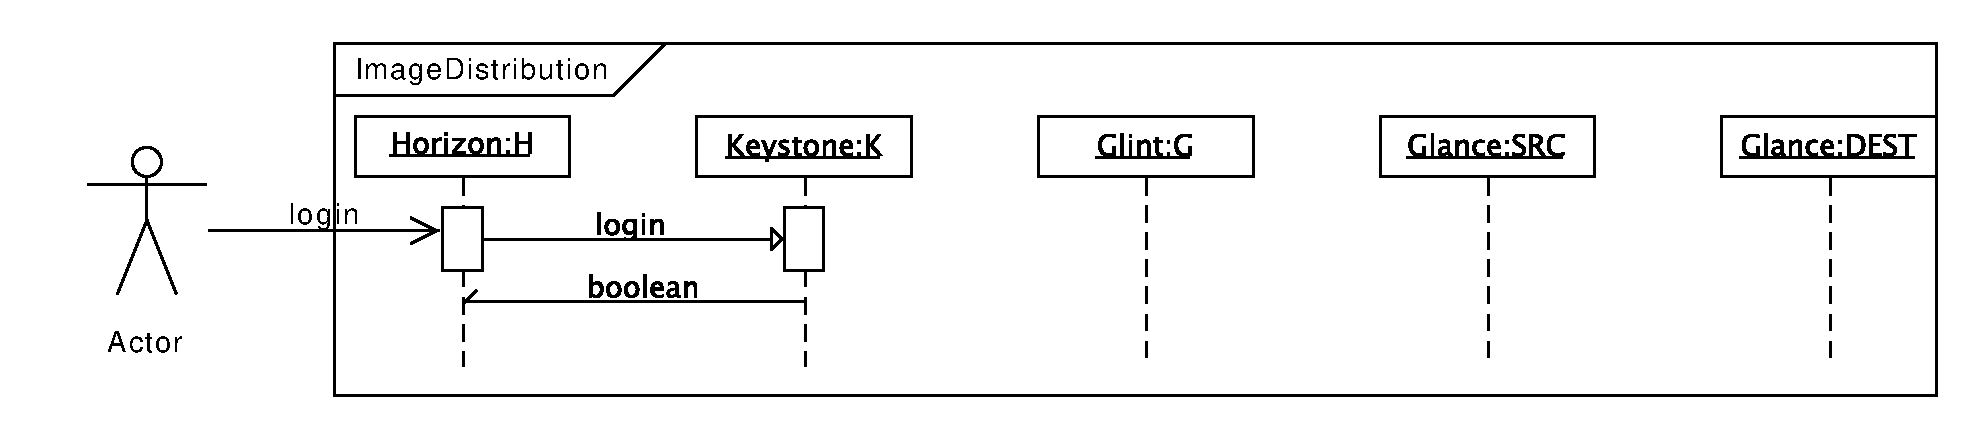
\includegraphics[width=36pc]{images/glintlogin.pdf}
\caption{\label{fig:glintlogin}Glint User Login}
\end{center}
\end{figure}

\begin{figure}[h]
\begin{center}
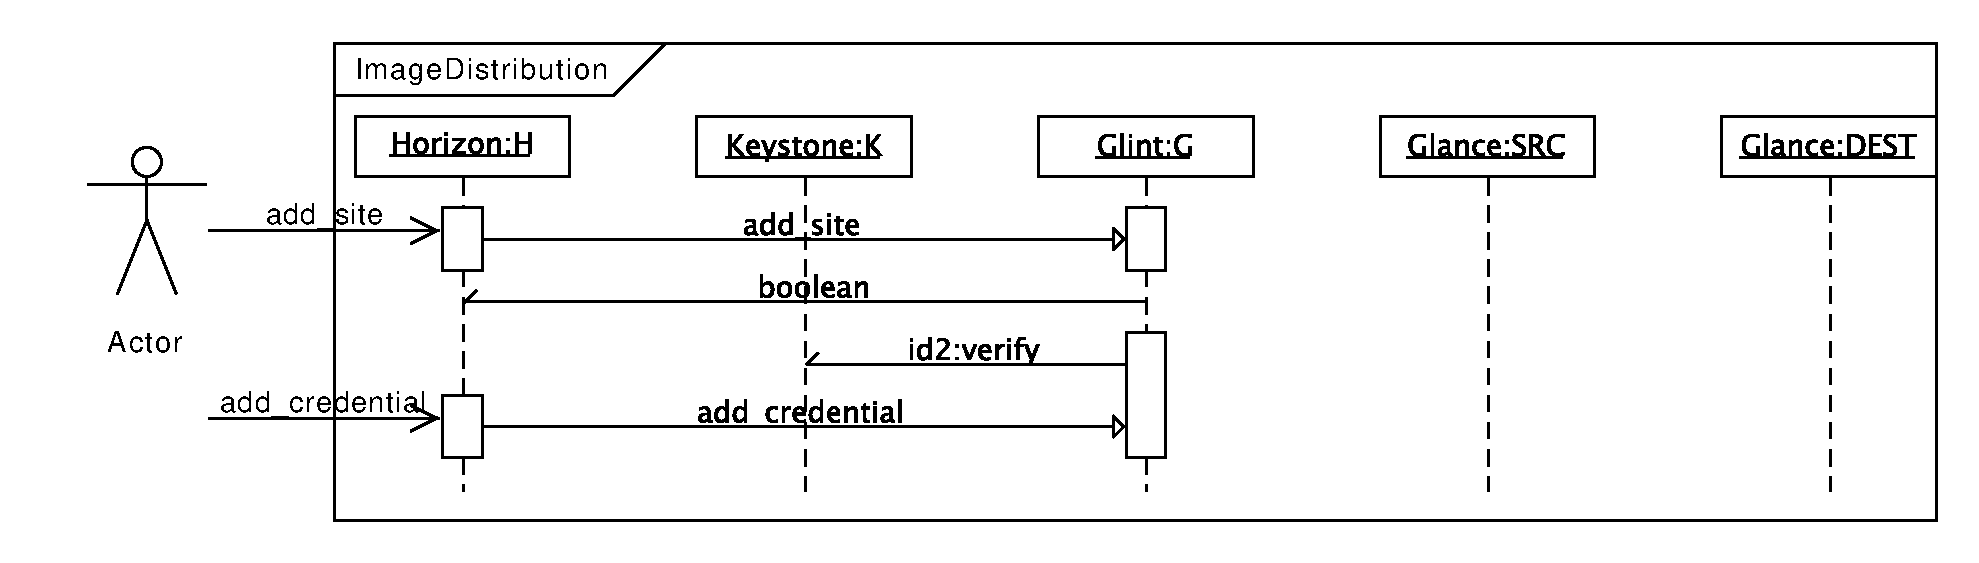
\includegraphics[width=36pc]{images/glintsitecred.pdf}
\caption{\label{fig:glintsitecred}Glint - Create remote site and add remote credential}
\end{center}
\end{figure}

\begin{figure}[h]
\begin{center}
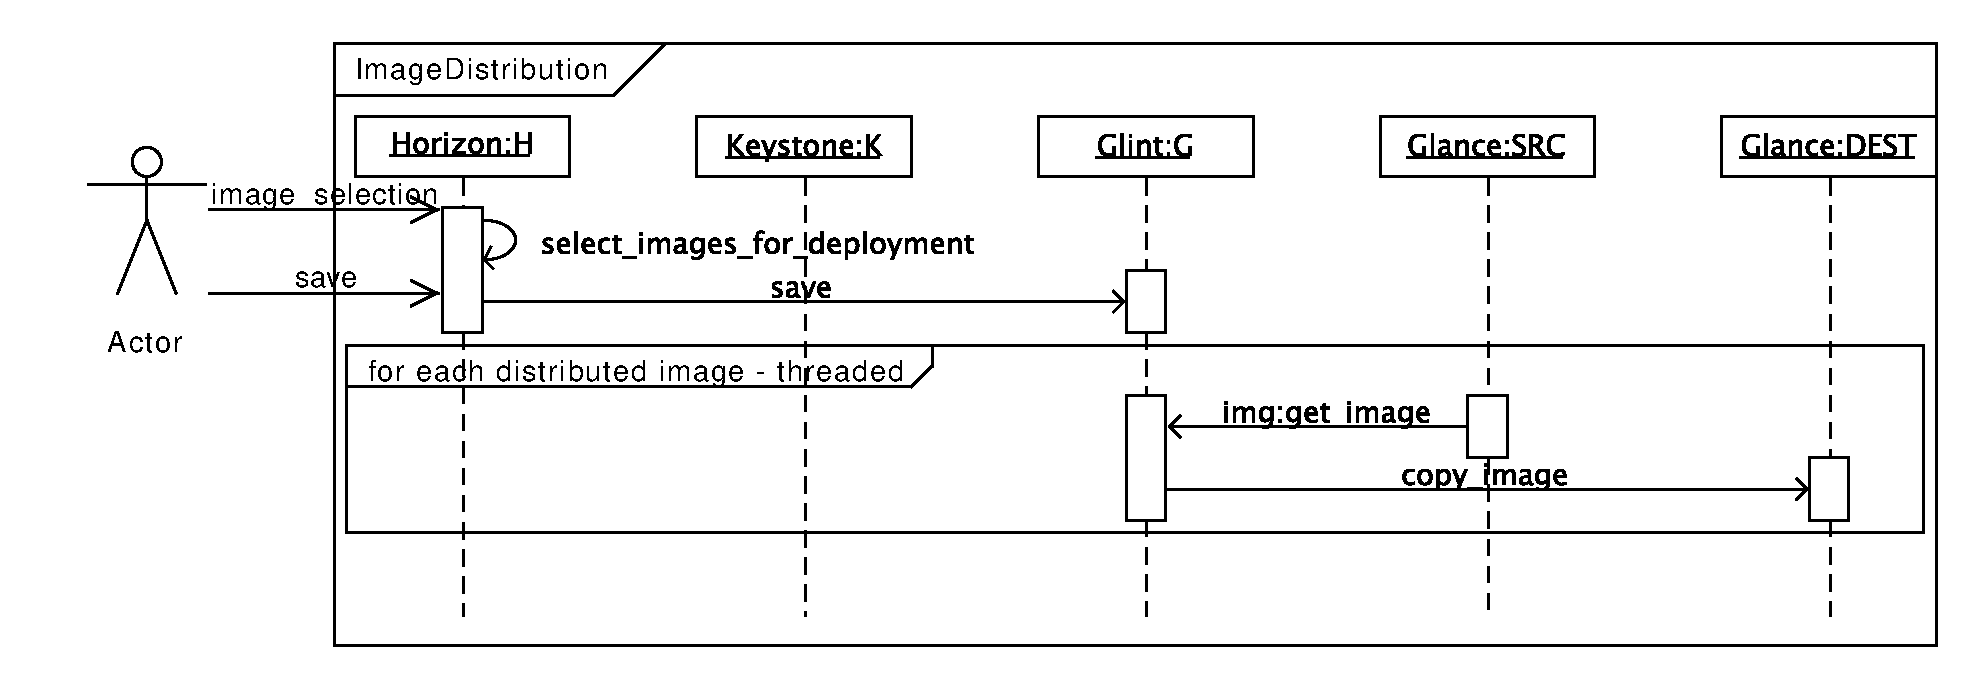
\includegraphics[width=36pc]{images/glintdist.pdf}
\caption{\label{fig:glintdist}Glint - Reconfigure Image Distribution}
\end{center}
\end{figure}

\section{Implementation}

Glint uses Django, a Python web framework, and the Data-Driven Documents (D3) 
JavaScript library toprovide users with an interface to manage their images and clouds. 
To communicate with the clouds, ituses Openstack’s Glance and Keystone API and Amazon’s Boto API. 
Python scripts use these API toolsto allow Glint to authenticate the users’ credentials with the 
cloud and then deploy and delete images fromeach cloud site. 
This design is illustrated in Figure 1



Django and D3 essentially create the server back-end and graphical interface front-end of the web service
respectively. 
These components use JSON formatted messages to send requests and responses to each other,such 
as getting the latest list of deployments or updating the newest list of deployments. 
Both parts of theinterface are well recognized products, as Openstack Horizon utilizes Django 
and D3 to design dashboards[6].

The basis for Django relies on models, where each user’s images, sites, and deployments are all 
stored ina model database [3]. 
For example, once an image and cloud site are stored in the database, the image could
be manipulated to deploy a new image onto a site, and then that new deployment is saved 
in the database forthat user. 
This is all done with Django’s built in Python API, but this database can be managed manually
using SQL queries as well [3].

The web service is designed so that each user has their own file system on the server where Django is
able to grab images and credential files, and there are measures to prevent the user from having duplicate images. 
Django also provides its own lightweight development server and a customizable administration
page, where the administrator can view and manipulate all users’ models with Django’s interface. 
From the3administration page, users can be given certain privileges to what they can access around the website [3],
and they can upload image and credential files on that page too instead of the Glint homepage.

The front-end of Glint is designed with D3, a Javascript library that presents the user interface and data
saved in Django for the user in an graphical representation. D3 still uses the basic web standards of HTML,
SVG, and CSS, but it utilizes functions which transform the user’s data to be interactive and have animated
transitions. 

These functions involve entering and exiting a selection of one’s data to modify individual orsets of nodes of data [2]. 
The Django and D3 tools thus provide the user with an appealing interface forusing Glint.


\section{Deployment}

With this interface, deploying an image onto a cloud is designed to be as simple as possible for the user. 
The user first uploads either an image file or a website address to a image file. 
To save an Openstack site, the user uploads the RC file and their password, and for 
Amazon Elastic Compute Cloud (EC2) sites, the useruploads their credentials to gain access to all EC2 regions. 
There is one extra step which requires the user to select their image to be bundled before being 
able to deploy onto EC2 sites. After the user has completed these steps, he or she is then ready to 
start managing all their images to be distributed to cloud sites.

Once the user has selected images to be 
deployed or deleted, the front-end will build the list in a JSON format by using a JSON message factory 
and give it an ‘update’ operation. 
Then it will send the list in an HTTP request to the Django server side, which then parses the JSON 
message and does the operation (inthis case, it is to update the current list of deployments). 
That ‘update’ message tells the back-end to filterthe deployments to either be deployed or deleted from 
Openstack or EC2.

When deploying on or deleting off Openstack, Glint uses Keystone and Glance Python API to obtain 
and gain access with security tokens to the Openstack cloud. 
Keystone represents the Openstack IdentityService by obtaining and verifying tokens using the values in 
the user’s RC file that was supplied earlier.
Tokens are also saved in the user’s database, and the web service will 
automatically update the token if it isexpired. Glance provides the tools for obtaining lists, creating, and 
deleting images on Openstack [5].

With EC2, Glint uses Boto, a Python interface for using Amazon Web Service tools. 
Boto is able to create and delete buckets to hold bundled images in Amazon’s Simple Storage Service (S3). 
Once the userhas selected a bundled image to deploy, it will upload the bundle to S3 
and then register the Amazon Machine Images (AMI) with EC2 [1]. 
And if the user is deleting an image, it will deregister the AMI and delete the bucket 
and its contents from S3.After Glint is finished updating the deployments it will store the image, site, 
and the UUID (or AMI idfor EC2 AMIs) from the image on the cloud in a deployed image model in the database. 
Then it sends thenew list back to the front-end in JSON. The HTTP utility there would get that response, 
parse the JSON message again, and present the new data to the user in D3.


\begin{figure}[ht]
\begin{center}
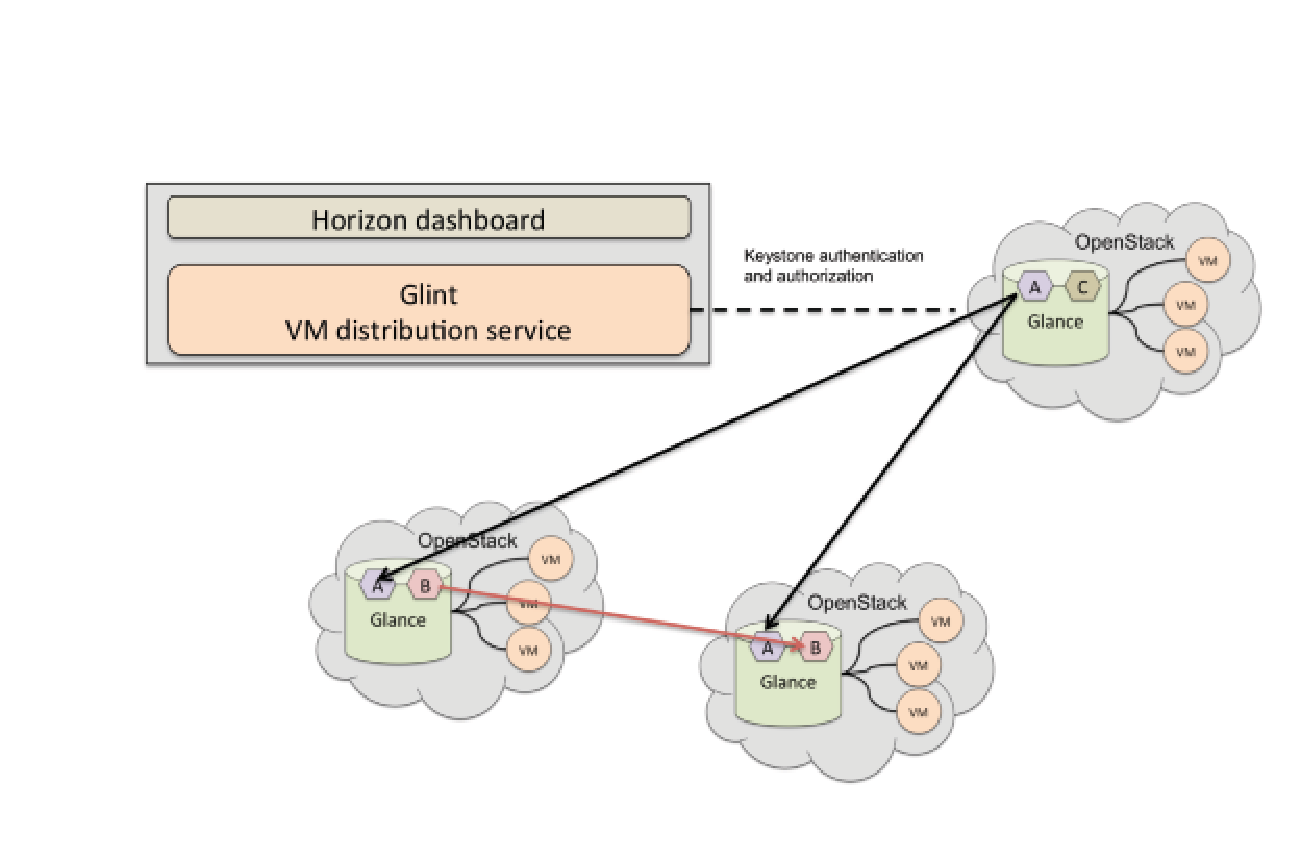
\includegraphics[width=36pc]{GlintFigure.eps}
\caption{\label{fig:glintfigure}An overview 
}
\end{center}
\end{figure}


%%% \newpage

\section*{References}
\begin{thebibliography}{9}

\bibitem{vmdirac}  
VM dirac

\bibitem{chep:gable-talk}
Gable chep talk

\bibitem{chep:vac-vcycle}
VAC vcycle

\bibitem{hpcs:cloudpaper}
HPCS cloud paper

\bibitem{sobie-nyc-cloud}
Sobie NYC talk

\bibitem{ryan-chep}
Ryan CHEP talk

\bibitem{sobie-chep}
Sobie Belle-II talk


\bibitem{glint}
{\it Glint}, a system for managing VM images on multiple clouds.
https://github.com/hep-gc/glint

\end{thebibliography}

\end{document}